
During our investigation, we had many frustrating experiences with existing research tools in this area.
These included installation issues, configuration issues, and dealing with unintuitive and undocumented interfaces.
For example, there are dozens of open issues without solutions on the VATIC GitHub,
and its installation script fails at multiple points on a brand new Ubuntu box.
Due to preciousness of researcher time,
we believe the ability for researchers to test and iterate quickly is just as important as worker speeds when it comes to video annotation.
Therefore we have placed improving the experimenter's experience as one of the main goals of this work.

\section{Interface for researcher}

BeaverDam provides a streamlined interface for a basic user creating a crowdsourced video dataset using the default configurations we provide.
We provide a setup script that is tested on clean installs of Ubuntu 14.04 and Ubuntu 16.04.
In comparison, VATIC was tested on an unspecified Ubuntu installation with exact Apache and MySQL installs,
and while the install script claims that it should work on any operating system in theory,
installation is difficult in reality.
Additionally, our install script configures everything from Nginx and TLS to database config and backups.
The user only needs to place their keys and credentials in the locations specified in our documentation.
While a containerization system such as Docker would have also solved VATIC's issues and ensure future compatibility,
we felt that the additional complexity is not worth it, as many of our users in the research community are unfamiliar with Docker.

To use BeaverDam after installation, we provide a web interface for researchers to easily add and view videos and jobs.
We feel that this is superior to VATIC's command line based approach,
as the number of flags needed to specify various configurations was overwhelming.
However, to allow experimenters to load large number of videos or perform other tasks programmatically,
BeaverDam also provides a Python shell interface, backed by Django, to expose every functionality through Python.

Lastly, as BeaverDam is HTML5 video based, no frame extraction step is necessary.
H.264 encoded videos will work without preprocessing. # H.264 is not a typo right?
However, we do provide scripts to convert these videos to images with matching annotations to feed into machine learning tools if desired.

\section{Decoupled modules}

As the users of BeaverDam will most likely need to modify BeaverDam to fit their needs,
we've emphasized modularity in our designs.
Since modularity is something VATIC did well with their turkic, vatic, and pyvision splits,
we've taken a similar approach.
Our infrastructure is split between a crowdsourcing module, an annotation module, and a CV-based tracking module.
But we decided to go a step further and make other parts of our platform replaceable as well.

To serve videos, we've provided Nginx to allow VATIC users to continue serving videos efficiently on the same server as their application.
But to allow for scalability, users can use AWS S3 or any other CDN, or even a mix, by specifying so when creating jobs.
Similarly, our setup pipeline is done through Ansible, a configuration management tool popular in industry.
This allows users to deploy on their own servers, or in the cloud.

We also understand that not everyone wants to use Amazon Mechanical Turk.
While past research has proven Mturk to be efficient and reliable,
companies in industry seeking training data may prefer alternatives such as CrowdFlower,
or may even choose to label in-house, or outsource to contractors.
BeaverDam is designed with this flexibility in mind as it carries its own authentication and works independently of Mturk.
This allows companies to use BeaverDam as a platform for their workers, no matter the type of labour, 
and track progress and pay without the need for Amazon Mechanical Turk, which carries a 20\% fee.

\begin{figure}[h]
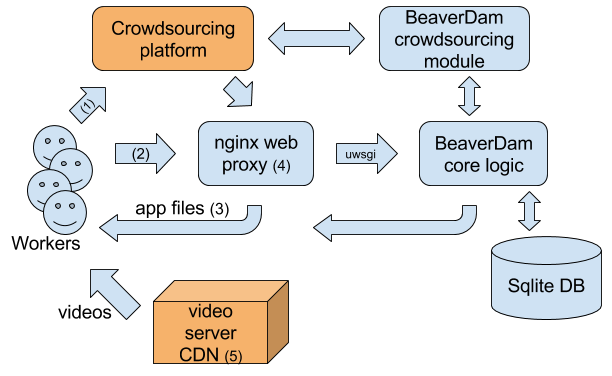
\includegraphics[width=14cm]{figs/backend.png}
\centering
\caption{BeaverDam's backend server logic. The annotation app is sent in (3). Workers can either be hired through a crowdsourcing platform (1), or hired in-house and use BeaverDam directly (2). The web proxy (4) smoothly handles many requests and forwards static files, and performs HTTPS authentication with HSTS to meet Mturk security requirements. A video server or cloud provider CDN (5) is used to reduce worker download waiting times, a problem of other video labeling tools.}
\end{figure}

\section{Patterns}

To facilitate modification of our code, we adopted the Django framework because it sets fairly strict conventions on how a project is structured.
Someone familiar with Django will immediate know where to find the files responsible for each function of the backend.
As there is a fair bit of frontend logic to video annotation, we've organized the code responsible according to well defined patterns as well.
Under Our Pattern Language ~\cite{opl}, the frontend follows the Model-View-Controller structure, and each of the three components is event-based.
While using events to communicate within an application may seem like additional complexity at first, it enables decoupling and extends the existing events from user interaction.

\section{Dependencies}

The number one problem we encountered during our installations of VATIC was broken dependencies.
Its GitHub issues point to problems users are having due to MySQL, cython, ipinfodb, and gcc versioning.
BeaverDam addresses this problem in two ways.
First, we greatly reduce the number of dependencies.
Python 3 and two python packages installed through pip are the only dependencies required to run BeaverDam.
Three other dependencies, Nginx, supervisor, and uwsgi, are recommended for efficient deployment.
And to avoid the burdensome installation and configuration of a database that VATIC required, we use sqlite3, which is a Python standard library.
In this case, it proves to be enough to handle even a fairly large amount of annotations, and can be swapped out easily if needed.
Second, we version each dependency.
This ensures that newer versions of dependencies in the future cannot break compatibility.
For front-end libraries, we check-in the required files directly instead of using a package manager, avoiding extra complexity.

Another problem we encountered with VATIC's dependencies was its system-wide installation and configurations.
Different users sharing a server would often leave bad state for others, causing hard-to-track bugs.
We enclose the project in a virtual environment, and we include an idempotent script that verifies all required state, and fixing them if necessary.
Our system is designed to be quickly set up on new VM instances,
so one can perform upgrades and fixes by discarding the entire server VM and starting from scratch.

When choosing our dependencies, we strived to use the latest versions of mature technologies.
We use Python 3.5 and Django 1.10, the latest versions available at the time.
We also use the ES6 version of JavaScript, which includes many features to enhance readability and programmer happiness.
While alternatives such as TypeScript provides additional features, ES6 is supported without a transpiler and avoids complexity.
Browser compatibility of ES6 was a small issue with workers, but we expect this to improve as browsers fully adopt the standard and workers update to the latest version of their browsers. # LOL IE6 4eva

\section{Security}

As BeaverDam aims to be industry quality software instead of research quality, security considerations are important.
While one would not expect malicious users, it's important to follow security best practices as a preventative measure.
Furthermore, having a full set of security tools allows the app to perform its own authentication,
adding to modularity by allowing it to function as a standalone app without Mechanical Turk, unlike VATIC.

The first and best line of defense is regular backups.
To back up data and configuration in VATIC, one had to perform a MySQL database dump and ensure all config files around the server are duplicated.
In BeaverDam, configuration is checked into version control, and the database is in a single file for easy backup and restore thanks to sqlite.
Our setup tool automatically sets a daily backup to Amazon S3 if the app is configured with access keys.
We also implemented other critical security features, such as TLS, HSTS, CSRF protection, and clickjacking protection. # out of curiosity, did you write these or are they from Django
These features are automatically installed and activated by our setup script,
with the user only needing to provide TLS certificates for their domain. \footnote{We recommend \textbf{letsencrypt} for easy and free TLS certificates.}


